\documentclass{article}
\usepackage{amsmath}
\usepackage{graphicx}
\usepackage{amssymb}
\begin{document}
\begin{enumerate}
    \item
        Let $u'(t) = 2t(1+u)$, $u(0)=0$. \\
        \begin{equation*}
            \begin{split}
                u_1(t) & = \int_{0}^{t} f(s, u(0))ds \\
                    & = \int_{0}^{t} f(s, 0)ds \\
                    & = \int_{0}^{t} 2sds \\
                    & = t^2 \\
            \end{split}
        \end{equation*}
        We can then derive $u_2$ and $u_3$:
        \begin{equation*}
            \begin{split}
                u_2(t) & = \int_{0}^{t} f(s, u_1(s))ds \\
                    & = \int_{0}^{t} f(s, s^2)ds \\
                    & = \int_{0}^{t} 2s(1+s^2)ds \\
                    & = \int_{0}^{t} 2s + \int_{0}^{t} 2s^3ds \\
                    & = t^2 + \dfrac{t^4}{2} \\
                u_3(t) & = \int_{0}^{t} f(s, u_2(s))ds \\
                    & = \int_{0}^{t} f(s, s^2 + \dfrac{s^4}{2})ds \\
                    & = \int_{0}^{t} 2s(1+s^2+\dfrac{s^4}{2})ds \\
                    & = \int_{0}^{t} 2s + \int_{0}^{t} 2s^3ds + \int_{0}^{t} s^5ds \\
                    & = t^2 + \dfrac{t^4}{2} + \dfrac{t^6}{6} \\
            \end{split}
        \end{equation*}
        It seems that the Picard iteration for this function takes the following pattern: \\
        \begin{equation*}
            \begin{split}
                u_k(t) & = \sum_{i=1}^{k} \dfrac{t^{2i}}{i!}
            \end{split}
        \end{equation*}
        Let $x=t^2$. Then the expanded series looks like a Taylor series: \\
        \begin{equation*}
            \begin{split}
                \lim_{k\rightarrow\infty}u_k(t) & = t^2 + \dfrac{t^4}{2!} + \dfrac{t^6}{3!} + ... \\
                \lim_{k\rightarrow\infty}u_k(x) & = x + \dfrac{x^2}{2!} + \dfrac{x^3}{3!} + ... \\
            \end{split}
        \end{equation*}
        It is known that $\sum_{n=0}^{\infty} \dfrac{x^n}{n!} = e^x$, so this sum converges to $u_{\infty}=e^{t^2}-1$. \\
    \item
        Let $x'(t) = f(t, x) = 1 + t - x(t)$, $x(0)=0$, $t_0=0$. Then, \\
        \begin{equation*}
            \begin{split}
                x_0(t) & = x(0) = 0 \\
                x_1(t) & = x_0 + hf(t_0, x_0) \\
                       & = 0 + h(1 + 0 - 0) \\
                       & = h \\
                x_2(t) & = x_1 + hf(t_1, x_1) \\
                       & = h + hf(h, h) \\
                       & = h + h(1 + h - h) \\
                       & = 2h \\
                x_3(t) & = x_2 + hf(t_2, x_2) \\
                       & = 2h + hf(2h, 2h) \\
                       & = 2h + h(1 + 2h - 2h) \\
                       & = 3h \\
            \end{split}
        \end{equation*}
        The series follows the pattern $x_n(t) = t_n$, so the original IVP is $x(t) = t$. \\
    \item
    \item
        See the source code at \texttt{https://github.com/codeandkey/math481-iastate-sp2020}. \\
    \item
        Here is the data collected from the program: \\
        \begin{center}
            \begin{tabular}{| c | c | c | c |}
                \hline
                $k$ & $U^N$ & $E^K$ & $E^{2K}/E^K$ \\
                \hline
                5e-2 & 38.093 & 15.505 & -- \\
                2.5e-2 & 44.846 & 8.752 & 1.771 \\
                1.25e-2 & 48.927 & 4.671 & 1.873 \\
                6.25e-3 & 51.182 & 2.417 & 1.933 \\
                3.125e-3 & 52.369 & 1.230 & 1.965 \\
                1.5625e-3 & 52.978 & 0.620 & 1.982 \\
                7.8125e-4 & 53.287 & 0.311 & 1.991 \\
                3.90625e-4 & 53.442 & 0.156 & 1.995 \\
                1.953125e-4 & 53.520 & 0.078 & 1.997 \\
                9.765625e-5 & 53.559 & 0.039 & 1.998 \\
                \hline
            \end{tabular}
        \end{center}
        Looking at this graph it is clear that as k tends towards infinity the error $E^N$ tends to 0.
        It appears that the ratio of $E^{2K}/E^K$ tends to 2, indicating that as k increases the error will halve on every increment. However, that improvement in error will quickly tend towards 0 as well.
    \item
        See the graph: \\
        \begin{center}
            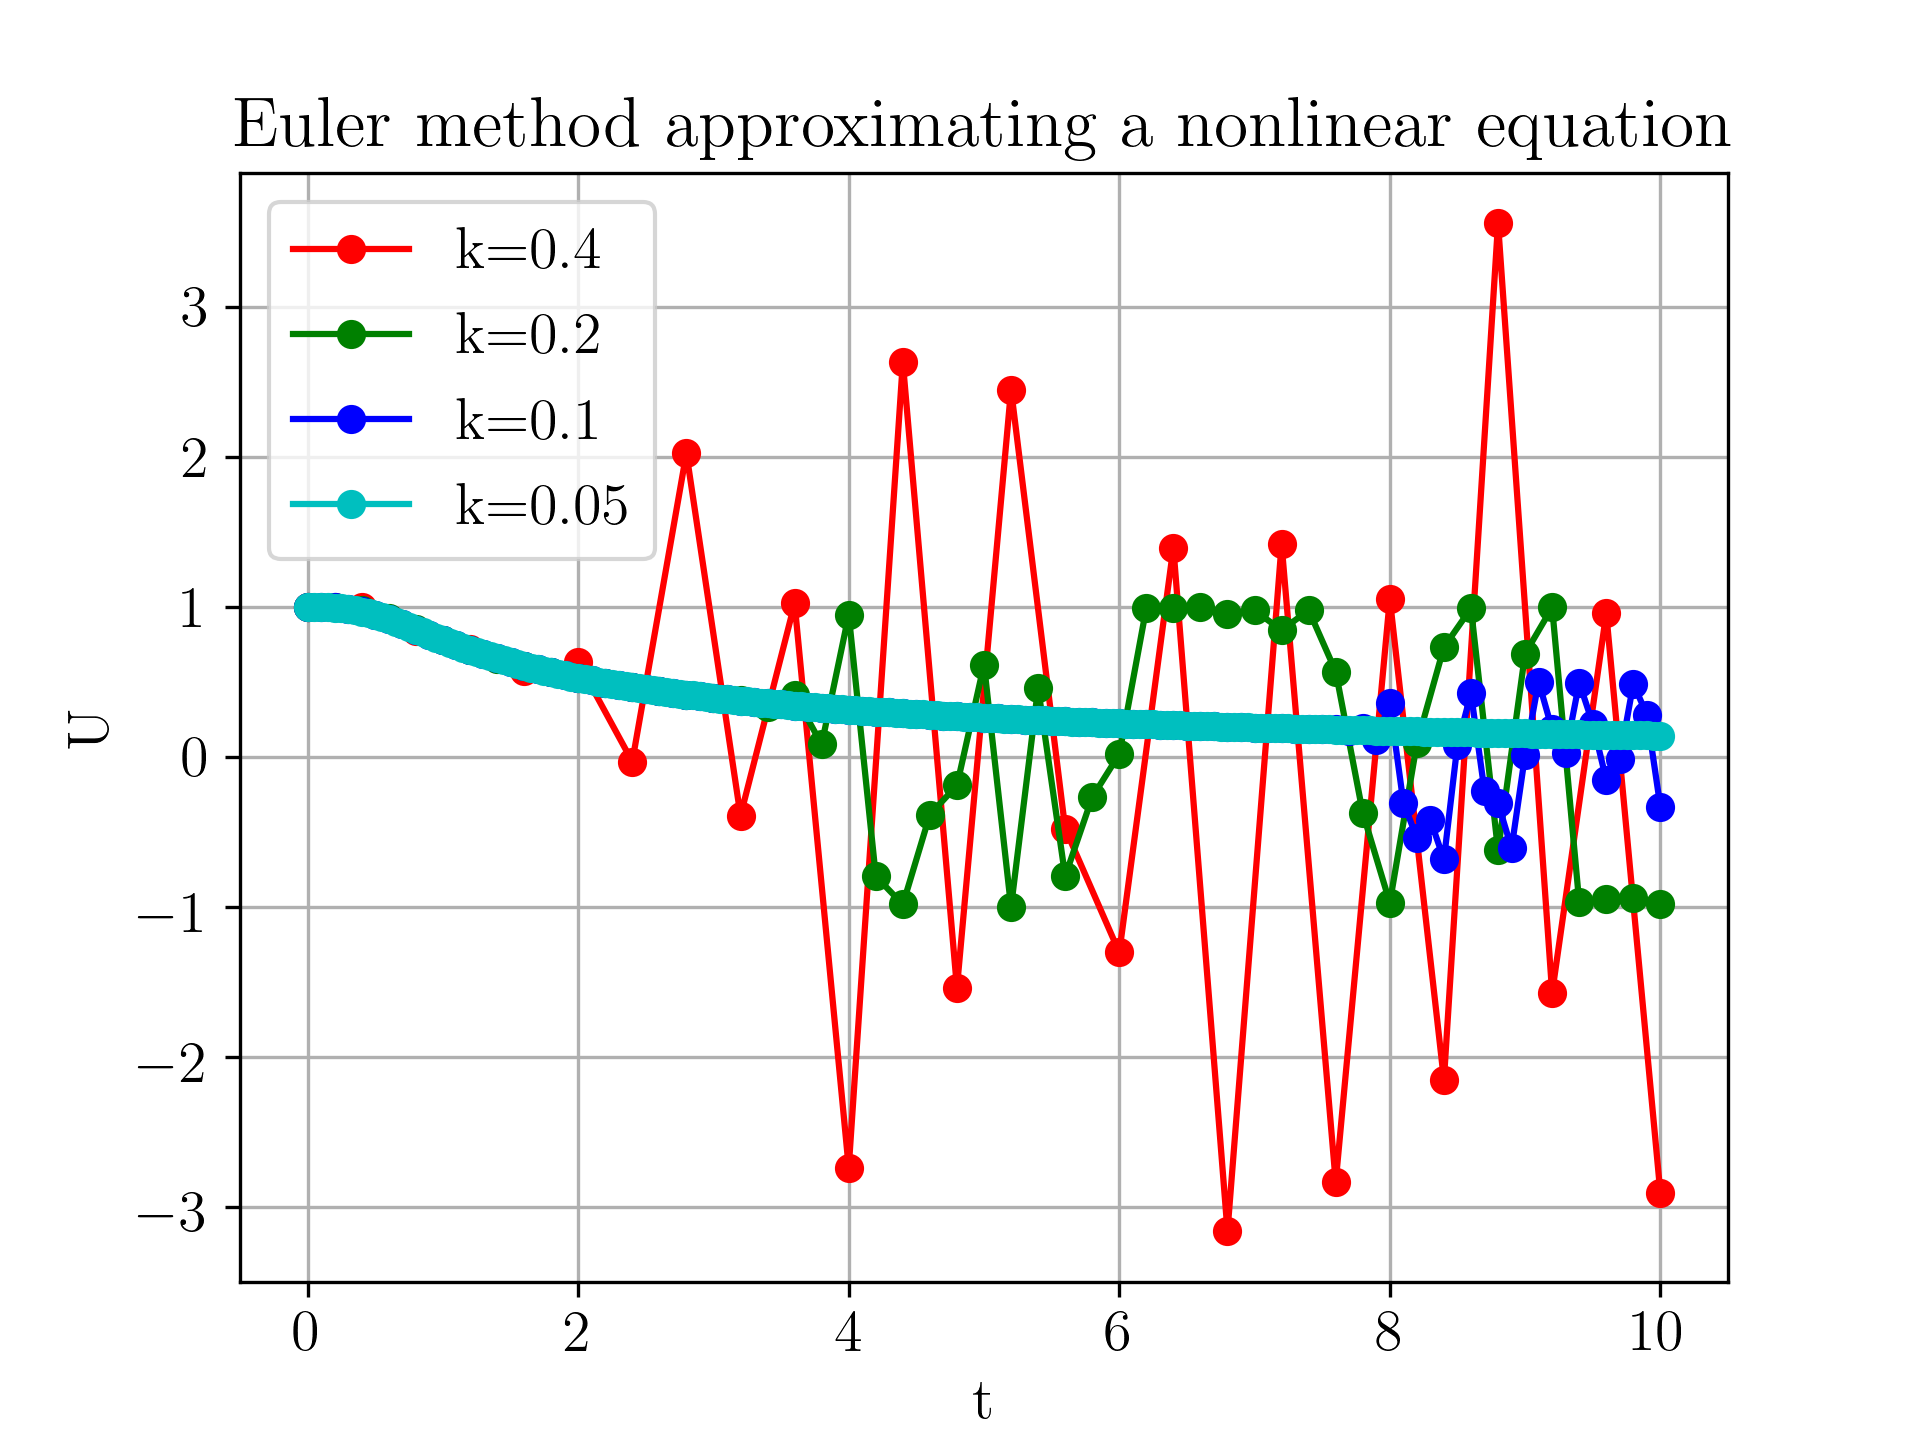
\includegraphics[width=0.75\textwidth]{q6.png}
        \end{center}
\end{enumerate}
\end{document}
